\section{РЕЗУЛЬТАТЫ РАБОТЫ}

\subsection{Результаты}
\label{section:results}

\subsubsection{Анализ методов разреженной регрессии}

Для анализа алгоритмов линейной регрессии при помощи \texttt{sklearn.datasets.make\_regression} сгенерирован датасет из 100 объектов, с одним значением целевой переменной. Каждый объект описывается 100 признаками, из которых значимыми являются только 10. К значениям признаков добавлен гауссовский шум с дисперсией 5. Визуализация истинных значений коэффициентов представлена на рисунке~\ref{fig:regr:coef}.

\begin{figure}
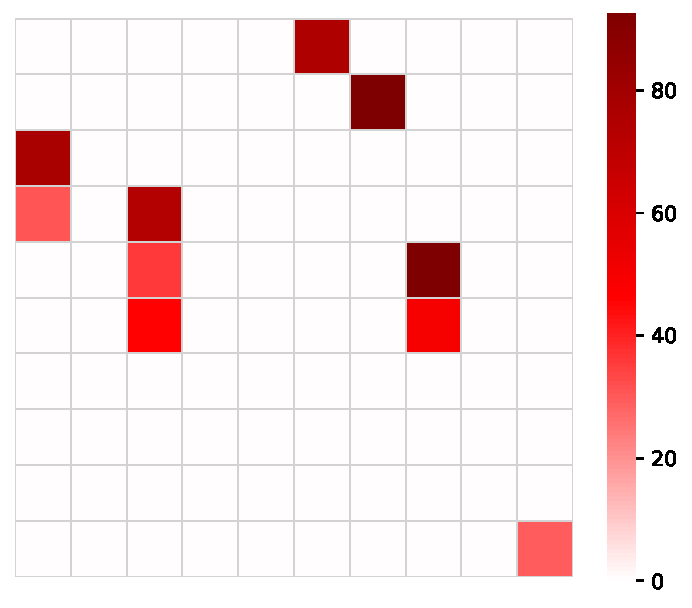
\includegraphics[width=.5\textwidth]{regr/coef}
\caption{Истинные коэффициенты}
\label{fig:regr:coef}
\end{figure}

В качестве контрольного примера, на рисунке~\ref{fig:regr:linear} приведены результаты работы обычной линейной регрессии без регуляризации. Для оценки результатов самой регрессии используются такие метрики, как максимальная ошибка, средняя абсолютная ошибка, среднеквадратичная ошибка, коэффициент детерминации. Как и ожидалось, такой метод хорошо предсказывает значения целевой переменной, но совершенно не справляется с отбором признаков. Хорошие результаты предсказаний также говорят о том, что этот метод подстраивается под шум.

\begin{figure}
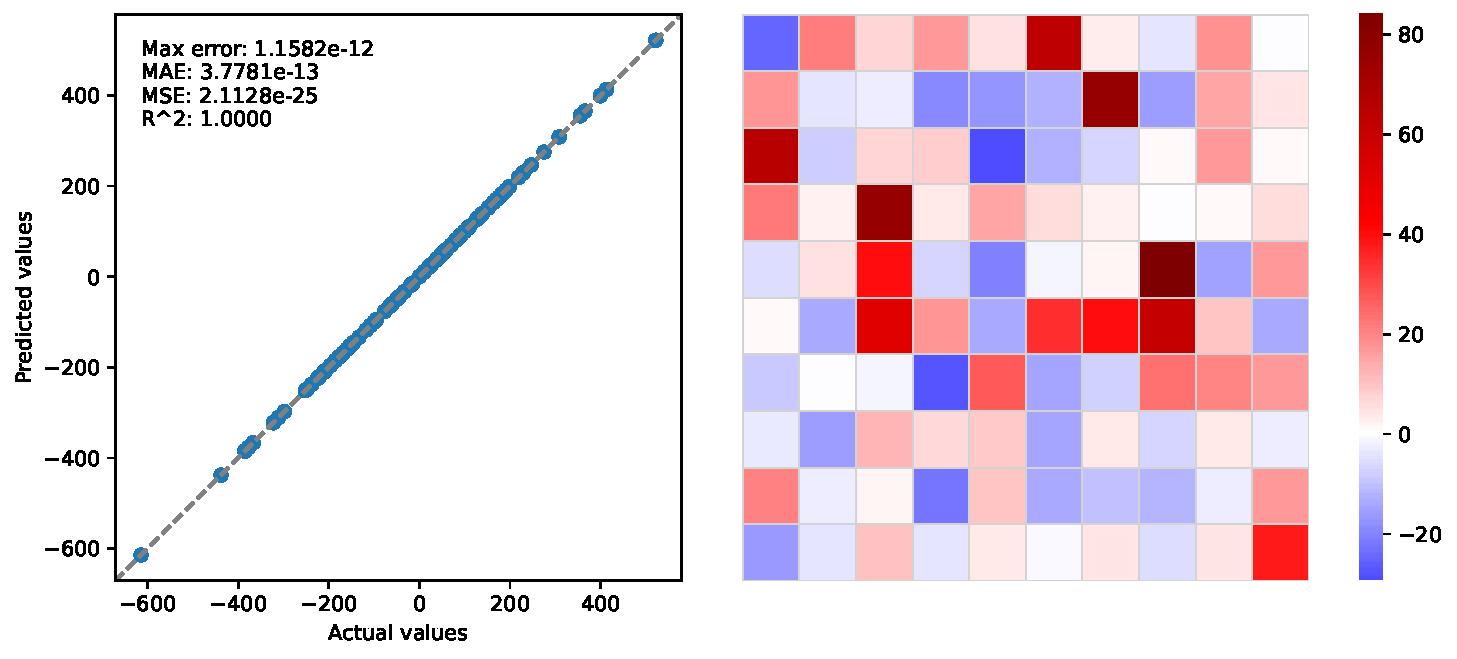
\includegraphics[width=\textwidth]{regr/linear}
\caption{Результаты работы линейной регрессия без регуляризации}
\label{fig:regr:linear}
\end{figure}

На рисунке~\ref{fig:regr:lasso} приведены результаты работы Lasso --- линейной регрессии с $L_1$ регуляризацией. Коэффициент регуляризации $\alpha = 1$.

\begin{figure}
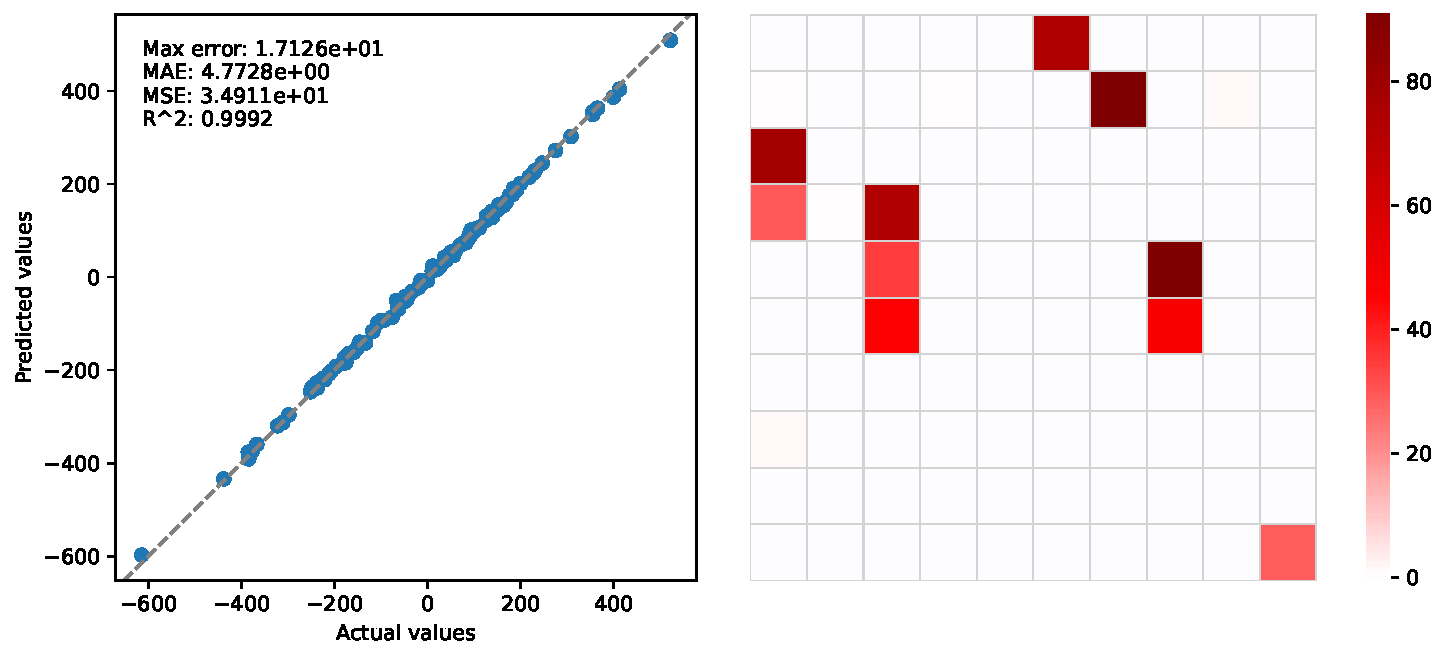
\includegraphics[width=\textwidth]{regr/lasso}
\caption{Результаты работы Lasso}
\label{fig:regr:lasso}
\end{figure}

На рисунке~\ref{fig:regr:stlsq} приведены результаты работы STLSQ. Пороговое значение $\alpha = 2$.

\begin{figure}
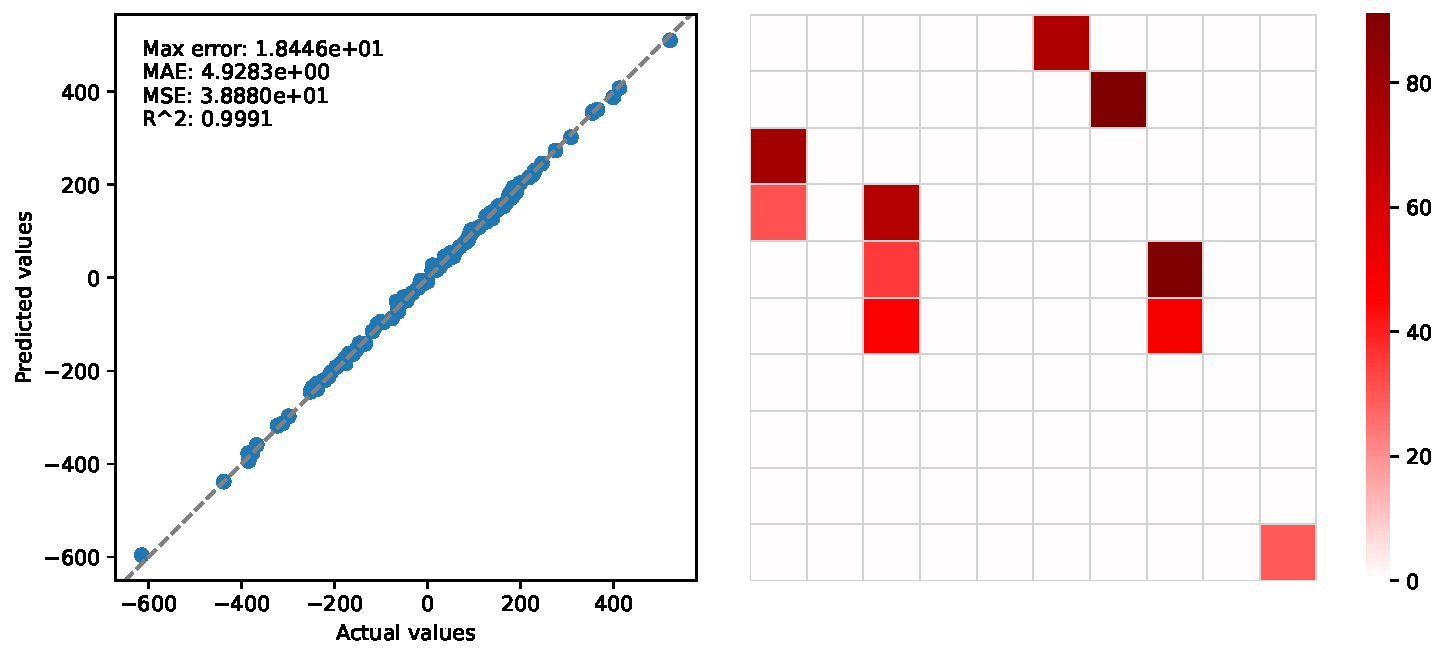
\includegraphics[width=\textwidth]{regr/stlsq}
\caption{Результаты работы STLSQ}
\label{fig:regr:stlsq}
\end{figure}

В результате тестирования можно сказать, что методы разреженной регрессии действительно справляются с поставленной задачей. Ценой этому служит необходимость подбора параметров и уменьшение точности. Но, так как они используются в структурной идентификации, отбор признаков является более важным результатом, чем качество предсказаний.
